\documentclass[a4paper,11pt]{article}

\usepackage[ngerman]{babel}

\usepackage{url}
\usepackage{abstract}
\usepackage{graphicx}
\usepackage{booktabs}
\usepackage{float}
\usepackage{tabularx}
\usepackage{amsmath}
\usepackage{hyperref}
\usepackage{listings}
\usepackage{color}
\usepackage{xcolor}
\usepackage{todonotes}
\usepackage{siunitx}
\usepackage{hyphenat}
\usepackage{fontspec}
\usepackage{todonotes}
\usepackage{longtable}
\usepackage{booktabs}
\usepackage{rotating}
\usepackage{pdflscape}
\usepackage{caption}
\usepackage{makecell}
%%\usepackage[bottom]{footmisc} breaks referencing of footnotes idk

\usepackage{tgpagella}
\setmainfont{TeX Gyre Pagella}

\usepackage[top=3cm]{geometry}
\usepackage{parskip} %% Absatz anstatt amerikanischer Einrückung

% configure vertical spacing in lists
\usepackage{enumitem}
\setitemize{partopsep=4pt,parsep=2pt}
\setdescription{partopsep=4pt,parsep=6pt}

\makeatletter
\def\namedlabel#1#2{\begingroup
#2%
\def\@currentlabel{#2}%
\phantomsection\label{#1}\endgroup
}
\makeatother

\definecolor{dkgreen}{rgb}{0,0.6,0}
\definecolor{gray}{rgb}{0.5,0.5,0.5}
\definecolor{mauve}{rgb}{0.58,0,0.82}

\lstset{
    numbers=none,
    language=SQL,
    frame=tb,
    captionpos=below,
    aboveskip=3mm,
    belowskip=3mm,
    xleftmargin=.01\textwidth, xrightmargin=.01\textwidth,
    showstringspaces=false,
    columns=flexible,
    basicstyle={\small\ttfamily},
    numberstyle=\tiny\color{gray},
    keywordstyle=\color{blue},
    commentstyle=\color{dkgreen},
    stringstyle=\color{mauve},
    breaklines=false,
    breakatwhitespace=true,
    tabsize=4
}

\newcommand{\shellcmd}[1]{\texttt{\footnotesize\$ #1}}

\newcommand{\localauthor}[1]{\color{gray} #1 \normalcolor}

\newcommand{\XXitem}[2]{\item[] \textbf{#1} \phantomsection \label{#2}}

\newcommand{\phantomLabel}[1]{\phantomsection\label{#1}}

\newcommand{\doubletitle}[2]{\title{#1 \\ [1ex] \normalsize #2}}
\newcommand{\extauthor}[2]{\author{#1 \\ \normalsize #2}}
\newcommand{\code}[1]{\texttt{#1}}

\begin{document}

    \begin{titlepage}
        \centering

        $~$

        \vspace{0.2cm} %% Hack for vspace to work

        \Huge \textbf{Validierungsbericht}\\

        \Huge Team 2
        \Large

        SEP WS 2021/22

        \vspace{2cm}

        
\includegraphics[width=0.8\linewidth]{graphics/LasEs-logo}

        \vspace{2cm}

        Betreuer:

        \textsc{Prof. Dr. Christian Bachmaier}

        \vspace{1cm}

        \begin{table}[H]
            \centering
            \Large
            \begin{tabular}{ll}
                \toprule
                \textbf{Projektphase} & \textbf{Leiter} \\
                \midrule
                Pflichtenheft & Johann Schicho \\
                Entwurf & Stefanie Gürster \\
                Feinspezifikation & Johannes Garstenauer \\
                Implementierung & Thomas Kirz \\
                Validierung & Sebastian Vogt \\
                \bottomrule
            \end{tabular}
        \end{table}

        \vspace{1cm}

        21. Januar 2021

    \end{titlepage}

    \pagenumbering{gobble}

    %%\maketitle
    \tableofcontents
    %%\listoftodos

    %% ENDE Titelblatt

    \newpage
    \pagenumbering{arabic}

    \section{Einleitung}\label{sec:einleitung}
    \localauthor{Johannes Garstenauer}


    \section{Integrationstests}\label{sec:integrationstests}
    \localauthor{Stefanie Gürster, Johann Schicho}

Wir verwenden das \emph{Selenium Framework} um mehrere Nutzerabläufe im Webbrowser zu automatisieren.
Dabei übernimmt ein Programm den Browser und navigiert anhand der \emph{ID}
der Webelemente. Dabei wird dann gegen die angezeigten Meldungen getestet, um
den korrekten Ablauf sicherzustellen.

\subsection{Probleme zu Beginn}

\begin{itemize}
	\item Verwendung von \emph{IDs} in JSF-Komponenten. Bereits während der
	Implementierung wurden überall, nach Definition der Feinspezifikation, IDs in den \emph{Facelets} verwendet.

	Allerdings wurde übersehen, dass auch \emph{Forms} und \emph{Composite Components} immer eigene IDs benötigen, da ansonsten JSF diese dynamisch
	generiert. Die dynamisch generierten IDs können sich bei jedem \emph{Render Vorgang} wieder ändern und erlauben damit also leider keine Identifikation.\newline
	Es wurden an allen Stellen, an denen die IDs vergessen wurden, diese noch eingefügt.



\end{itemize}

    \section{Stresstest}\label{sec:stresstest}
    \localauthor{Sebastian Vogt}

\subsection{Versuchsaufbau}

\subsubsection{Beteiligte Geräte}
\begin{itemize}
	\item Der FIM Rechner bueno als Referenzsystem für den Datenbankserver
	\item Der FIM Rechner ds9 als Referenzsystem für den Tomcat-Server.
	\item Der FIM Rechner galactica als System für die Latenzmessungen.
	\item Die drei Entwicklerlaptops \emph{Lenovo IdeaPad Flex 5 14IIL05} (kurz \textbf{Lenovo5}), \emph{Lenovo IdeaPad C340-14IML} (kurz \textbf{LenovoC}) und \emph{Acer Aspire A515-54G} (kurz \textbf{Acer}), wie im Pflichtenheft spezifiziert. Diese haben über das Bayern-WLAN an der Universität Passau und VPN auf den Webserver zugegriffen.
\end{itemize}

\subsubsection{Messung der Antwortzeiten}\label{sec:mess}
Wir haben uns dafür entschieden, die Messung der Antwortzeiten auf einem Rechner in der FIM zu machen. Dies hat folgende Vorteile:
\begin{itemize}
	\item Die Stressoren und der Messungsrechner sind nicht im selben Netwerk, d.h. die von den Stressoren generierte Auslastung des Netzwerks wird vom Messungsrechner nicht mitgemessen
	\item Da der Messungsrechner im selben Netzwerk ist wie der Webserver, verfälscht die Internetverbindung des Messungsrechners nicht das Ergebnis.
	\item Da der Messungsrechner und die Stressoren verschieden sind, verfälscht die Auslastung der Stressoren selbst durch die Belastungstests nicht das Messergebnis.	
\end{itemize}
Natürlich hat diese Entscheidung einen Nachteil:\\
 Die im Pflichtenheft geforderte Antwortzeit von maximal 3 Sekunden bezieht sich auf den Endnutzer, aber in den Messdaten fehlt die Propagationszeit zwischen dem Endnutzer und dem Universitätsnetzwerk. Es ist wohl eine sinnvolle Annahme, dass eine Verdreifachung der Messwerte diesen Effekt im Mittel ausgleicht. Also müssen wir im folgenden Überprüfen, dass unsere Messwerte unter einer Sekunde liegen.

\subsubsection{Software}

Für die Lasttests wurden zwei gängige Nutzerflüsse auf LasEs mit Selenium automatisiert:
\begin{itemize}
	\item Nutzerfluss 1: Hier registriert sich ein neuer Nutzer im System, navigiert eine Zeit lang im System und löscht dann sein Konto wieder.
	\item Nutzerfluss 2: Hier wird ein neues wissenschaftliches Forum erstellt, eine neue Einreichung erstellt und eine Revision angefordert und eingereicht.
\end{itemize}
In der Browserautomatisierung wird bei jedem HTTP-Request die Antwortzeit des Servers gemessen und zusammen mit Kontextinformation über die ausgeführte Interaktion abgespeichert. Diese Testsuite wurde auf den Stressoren und dem Messungsrechner ausgeführt.

Dabei gab es zwei Konfigurationen, bei denen die Testsuite je folgendermaßen ausgeführt wurde:

\paragraph{Konfiguration 1: 30 Stressoren}
\begin{itemize}
	\item \textbf{Lenovo5}: 7 parallele Ausführungen von Nutzerfluss 1 und gleichzeitig 8 parallele Ausführungen von Nutzerfluss 2
	\item \textbf{LenovoC}: 7 parallele Ausführungen von Nutzerfluss 1 und gleichzeitig 8 parallele Ausführungen von Nutzerfluss 2
\end{itemize}

\paragraph{Konfiguration 2: 50 Stressoren}
\begin{itemize}
	\item \textbf{Lenovo5}: 7 parallele Ausführungen von Nutzerfluss 1 und gleichzeitig 8 parallele Ausführungen von Nutzerfluss 2.
	\item \textbf{LenovoC}: 10 parallele Ausführungen von Nutzerfluss 1 und gleichzeitig 10 parallele Ausführungen von Nutzerfluss 2.
	\item \textbf{Acer}: 7 parallele Ausführungen von Nutzerfluss 1 und gleichzeitig 8 parallele Ausführungen von Nutzerfluss 2.
\end{itemize}

\paragraph{Konfigurationsunabhängig\\}
Bei beiden Konfigurationen wurde auf den restlichen Rechnern je folgendes ausgeführt:
\begin{itemize}
	\item Der Messungsrechner führt jeden Nutzerfluss einmal parallel aus und speichert danach die Antwortzeitmessungen in einer CSV Datei.
	\item Application Server und Datenbankserver führen das LasEs System auf Tomcat und die PostgreSQL Datenbank aus.
\end{itemize}

\subsection{Ergebnisse}

Bei beiden Konfigurartionen wurden für eine Reihe verschiedener Nutzerinteraktionen Messwerte aufgezeichnet. Meistens existiert pro Nutzerinteraktion ein Messwert. Wenn zwei oder drei Messwerte existieren, wurde im folgenden Balkendiagramm jeweils der größte Messwert aufgenommen. Alle Messwerte werden in Millisekunden angegeben. In \hyperref[fig:worst30]{Abbildung 1} findet sich das Balkendiagramm für Konfiguration 1, in \hyperref[fig:worst50]{Abbildung 2} findet sich das Balkendiagramm für Konfiguration 2.

\begin{figure}[H]
	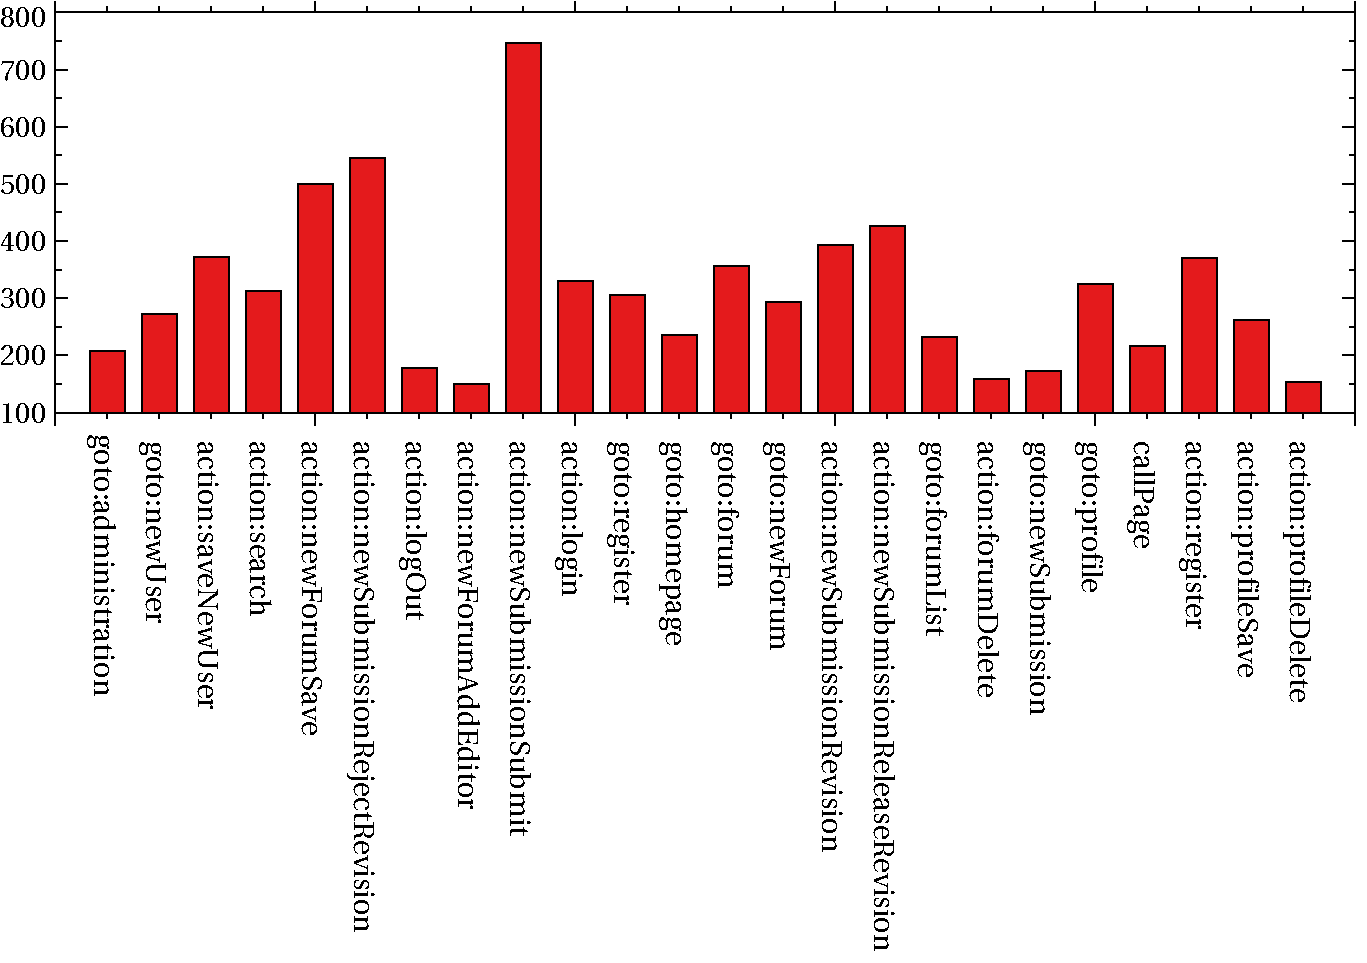
\includegraphics[width=\linewidth]{graphics/30worstcase.pdf}
	\caption{Konfiguration 1}
	\label{fig:worst30}	
\end{figure}
\begin{figure}[H]
	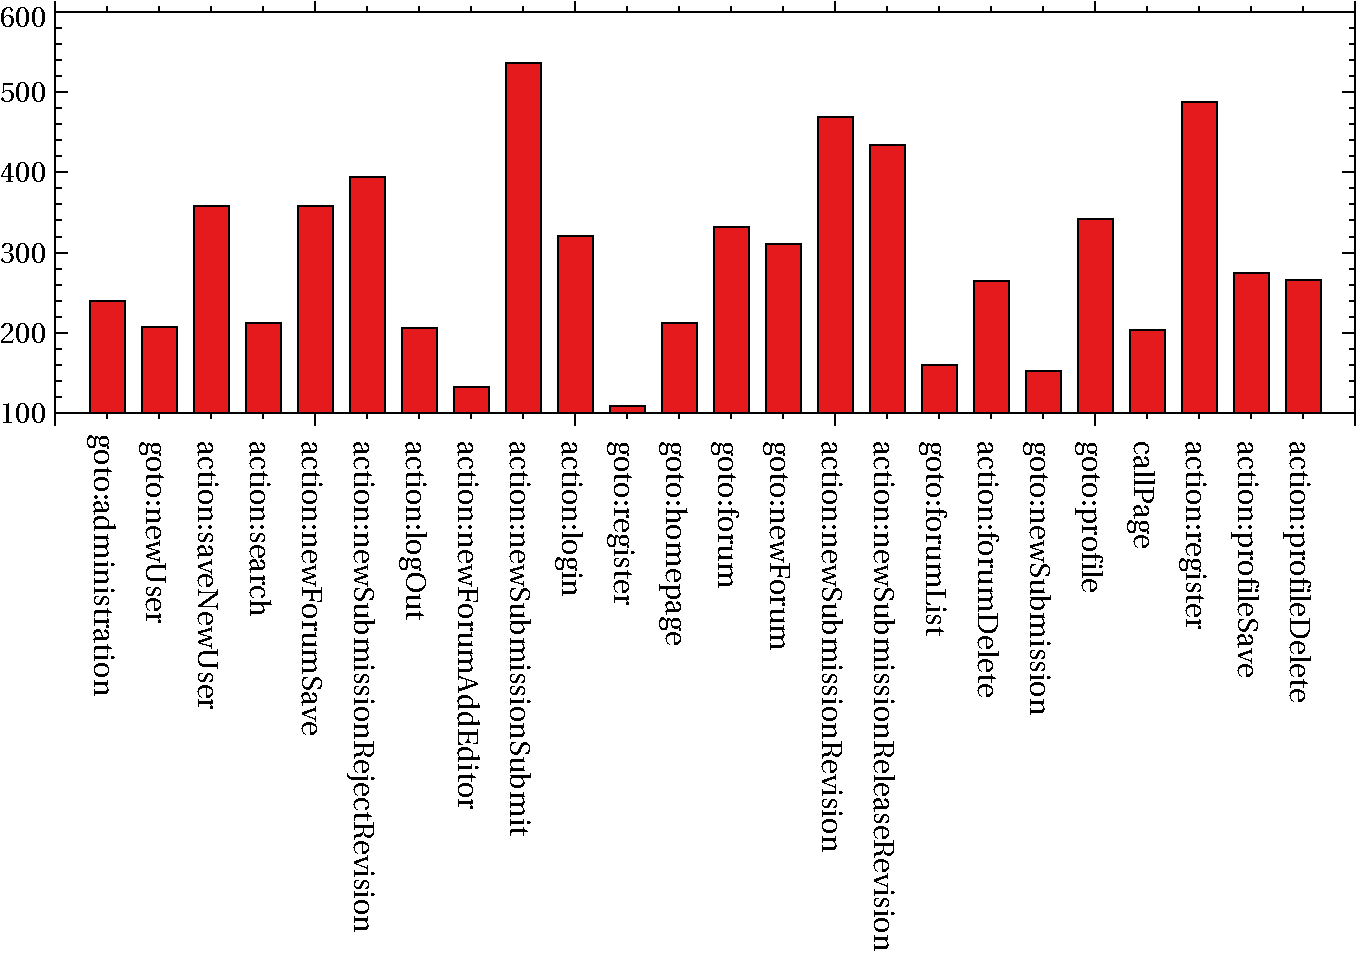
\includegraphics[width=\linewidth]{graphics/50worstcase.pdf}
	\caption{Konfiguration 2}
	\label{fig:worst50}	
\end{figure}

In \hyperref[fig:boxplot]{Abbildung 2} sieht man einen Boxplot, der die Werte der zwei Konfigurationen vergleicht. Im Boxplot zeigen die Whisker das 9/91 Perzentil. Der Kreis in der Box ist jeweils der Mittelwert. Die Kreise außerhalb sind alle Messwerte, die nicht innerhalb des Wertebereichs der Whisker liegen.

\begin{figure}[H]
	\includegraphics[width=\linewidth]{graphics/boxplots.pdf}
	\caption{Boxplot}
	\label{fig:boxplot}	
\end{figure}


\subsection{Interpretation}

Alle Zeitmessungen befinden sich im Bereich unter einer Sekunde, insbesondere bei 50 gleichzeitigen Nutzern. Wie im Bereich \hyperref[sec:mess]{Messung der Antwortzeiten} begründet, erfüllt dies die Skalierbarkeitsanforderung des Pflichtenhefts.

Die langsamste Nutzerinteraktion war in beiden Konfigurationen das Einreichen einer neuen Einreichung. Dies war bereits in der Entwicklungsphase abzusehen, da die Einreichungsseite eine große Menge an Daten anzeigen und somit laden muss.

Interessanterweite ist die Ausführung bei 50 Nutzern im Median nur verschwindend langsamer, im Durchschnitt sogar schneller als bei 30 Nutzern. Dies ist vielleicht dadurch zu erklären, dass bei 50 Nutzern die Ausführung der Stressoren auf einem der drei Laptops in einigen Threads sehr schnell zu Fehlern geführt hat und neugestartet werden musste. Dies führt uns auch schon zum letzten Punkt, und zwar den einschränkenden Bedingungen dieser Untersuchung.

\subsection{Einschränkungen}

Die Ausführung der Stressoren war sehr instabil. Dies ist auf zwei Gründe zurückzuführen. Einerseits ist die Ausführung der Selenium-Routinen oft plattformabhängig. Nicht nur das Betriebssystem, sondern auch verschiedene Hardwarekonfigurationen führen dazu, dass eine Operation auf einem Rechner fehlschlägt und auf einem anderen nicht. Andererseits stießen die verwendeten Laptops bei der Ausführung der Stresstest sehr schnell an ihre eigenen Belastungsgrenzen, was dazu führte, dass einzelne Threads wegen Zeitüberschreitung mit einer Selenium Exception endeten. Diese brachten dann narürlich den ganzen Ausführungsthread zum erliegen, wodurch ein simulierter Nutzer verloren ging.

Als zweiter einschränkender Faktor ist natürlich die Näherung der tatsächlichen Endnutzer Antwortzeit durch das Dreifache unserer Antwortzeit zu nennen. Im Idealfall würde die Antwortzeit durch einen seperaten Rechner, der sich in einem anderen Netz als die Stressoren oder der Webserver befindet, durchgeführt.



    \section{Sicherheitstests}\label{sec:sicherheitstests}
    \localauthor{Thomas Kirz}

Zusätzlich zu den Tests aus dem Pflichtenheft wurden folgende Tests geschrieben,
um verschiedene Sicherheitsaspekte des Systems zu testen.

\subsection{Injection}\label{subsec:injection-test}
Dieser Test prüft den Schutz gegen SQL- und HTML/JavaScript-Injection.

Dazu wird ein Nutzerkonto angelegt mit dem Titel \emph{;DROP table user;--}.
Wäre hier SQL-Injection möglich, würde dieser Titel bei Ausführung des \code{INSERT}-Statements in der Datenbank
die \code{user}-Tabelle löschen.

Dann lädt der Nutzer eine Einreichung mit dem Titel \emph{<script>alert('XSS');</script>} hoch.
Der Titel soll jetzt so wie eingegeben angezeigt werden, ohne dass JavaScript ausgeführt wird.

\subsection{Aufruf ohne Login}\label{subsec:unauthorized-test}
Ohne anzumelden, wird versucht, die Startseite (für authorisierte Nutzende) aufzurufen.
Der Nutzer soll auf die Anmeldeseite weitergeleitet werden.

\subsection{Session Fixation}\label{subsec:session-fixation-test}
Für diesen Test werden Cookies deaktiviert, damit die Session-ID in die URL geschrieben wird.

Ein Nutzer ruft die Webseite auf und bekommt eine Session-ID\@.
Mit dieser Session meldet er sich an.
Wird die Webseite nun erneut mit der alten Session-ID aufgerufen, darf der Nutzer nicht angemeldet sein.

\subsection{Insecure Direct Object Reference}\label{subsec:idor-test}
Dieser Test prüft, dass ein Nutzer nicht unberechtigt auf Inhalte zugreifen kann, indem er deren ID herausfindet.

Dazu legt ein angemeldeter Nutzer eine Einreichung an.
Ein weiterer, neu registrierter Nutzer versucht jetzt,
die Seite für diese Einreichung (mit richtiger ID als URL-Parameter) aufzurufen.
Die Einreichung darf nicht angezeigt werden.


    \section{Testmetriken}\label{sec:testmetriken}
    \localauthor{Johannes Garstenauer}

Im Folgenden soll die Qualität der Testsuites bestimmt werden,
um ihre Aussagekraft hinsichtlich der Bestätigung der Qualität des LaSes\-System zu evaluieren.
Hierzu wird die Quelltextüberdeckung der \emph{Unittests} sowie der \emph{Integrationstests} untersucht.
Schlußendlich werden die Ergebnisse interpretiert.

\subsection{Quelltextüberdeckung}\label{subsec:quelltextueberdeckung}
Zur Messung der Quelltextüberdeckung wurde die populäre \emph{Java Code Coverage Library \textbf{JaCoCo}} verwendet.
In der Analyse wird ein besonderes Augenmerk auf die Werte der \emph{Zeilen-} und \emph{Zweigüberdeckung} gelegt,
da diese am aussagekräftigsten bezüglich der Testqualität sind.

\subsubsection{Unit Tests}
Es existieren \emph{Whiteboxtests} zu den meisten Klassen und Methoden des Projekts.
Es besteht jedoch kein Anspruch auf Vollständigkeit.
Die \emph{Unittests} entstanden größtenteils parallel zur Entwicklung.
Bestimmte Arten von Klassen wurden hierbei ausgespart:

\begin{itemize}
    \item \emph{Backing-Beans}: Es bestand die Erwartung, dass diese sinnvoller in den \emph{Blackboxtests}
    abgedeckt werden können.
    \item \emph{Klassen in den internal-Paketen}: Hier war in der Regel ein großer \emph{Mockingaufwand} vonnöten,
    um erwartetes Verhalten testen zu können.
    Dies liegt an der großen Anzahl von \emph{Jakarta Server Faces} spezifischen Komponenten,
    welche in diesen Klassen verwendet werden.
    Aufgrund des Wunsches, vonseiten der Entwickler, die begrenzte Entwicklungszeit
    wirkungsvoll einzusetzen und der oft überschaubaren \emph{JSF}\-fremden Logik, welche zu überprüfen war,
    wurden diese Klassen beim \emph{unittesting} oft ausgespart.
    Beispiele hierfür sind z.B. der \emph{UncheckedExceptionHandler} oder \emph{MessageResourceBundleProducer}.
\end{itemize}
Die \emph{Quelltextüberdeckungswerte} sind vor diesem Hintergrund zu betrachten.

\begin{figure}[h]
    \centering
    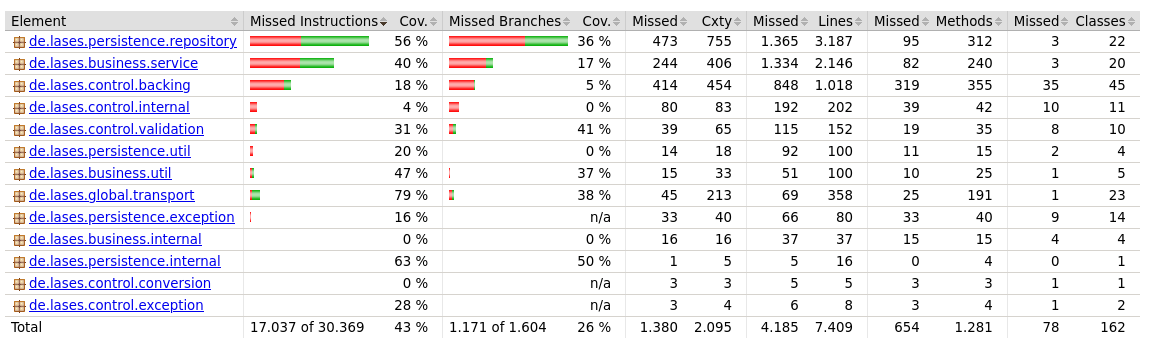
\includegraphics[width=0.9\linewidth]{graphics/coverage_unit}
    \caption{Übersicht über die genauen Überdeckungswerte (gegliedert nach Paketen)}
    \label{fig:coverage_unit}
\end{figure}

Die 96 Testmethoden der Unittests erreichen eine \emph{Zeilenüberdeckung} von \textbf{43\%}
und eine \emph{Zweigüberdeckung} von \textbf{26\%}.


\subsubsection{Integration Tests}
Die \emph{Blackboxtests} decken große Teile der vorgesehenen Funktionalität ab und beinhalten zusätzlich Tests
zu sicherheitskritischen Szenarien, wie \emph{Skript- und Sequelinjektionen}.
Es besteht wiederum kein Anspruch auf Vollständigkeit.
Erwartete Schwachstellen der \emph{Quelltextberdeckung} sind zu erwarten aufgrund von:
\begin{itemize}
    \item Den entgegengesetzten Prinzipien von \emph{Isolation} und \emph{Integration} im Software Testing.
    Integrationstests weisen eine höhere Integration (d.h. ein höheres Clustering der Features in den Tests)
    auf Kosten der Isolation auf und erreichen aufgrunddessen weniger Granularität, beispielsweise in der Zweigabdeckung.
    Daraus resultiert eine geringere \emph{Quelltextüberdeckung}.
    \item Codeabschnitte, welche sich der defensiven Programmierung widmen, werden seltener überdeckt
\end{itemize}
Die \emph{Quelltextüberdeckungswerte} sind vor diesem Hintergrund zu betrachten.

Die Integrationtests erreichen eine \emph{Zeilenüberdeckung} von \textbf{45\%}
und eine \emph{Zweigüberdeckung} von \textbf{34\%}.

\begin{figure}[h]
    \centering
    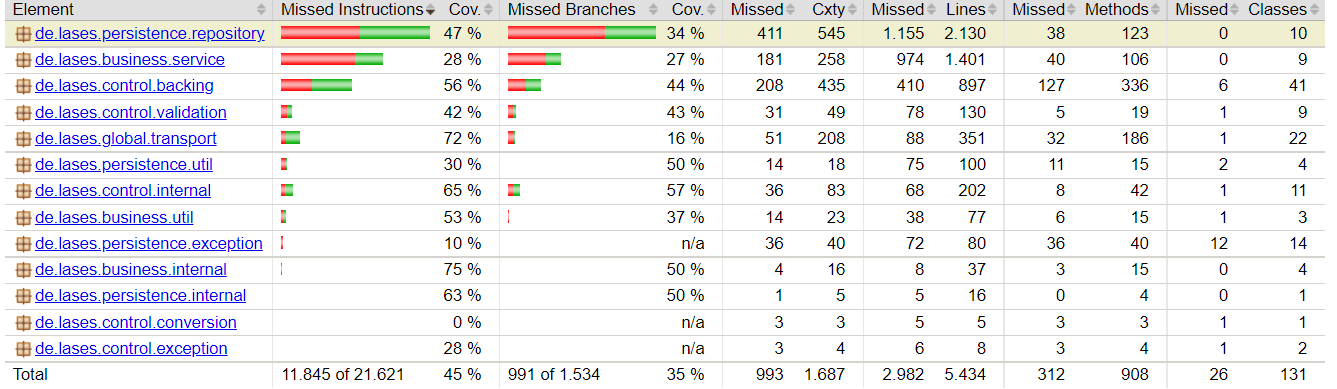
\includegraphics[width=0.9\linewidth]{graphics/coverage_it}
    \caption{Übersicht über die genauen Überdeckungswerte (gegliedert nach Paketen)}
    \label{fig:coverag_it}
\end{figure}

\end{document}
